%----------------------------------------------------------------
%
%  File    :  survey-animation.tex
%
%  Author  :  Keith Andrews, IICM, TU Graz, Austria
% 
%  Created :  27 May 1993
% 
%  Changed :  03 Feb 2017
% 
%----------------------------------------------------------------


\chapter{Animated Slideshow}

\label{chap:animated}

The biggest downside of the original \textit{rSlidy} when compared to alternative solutions, with focus on well spread desktop solutions, would be its static state. Namely the presentation flow achieved with the application was an immediate switch between states or slides. Even the user interface was behaving similarly in a state-switching way. In the design changes the effects of hiding elements with hover and transition CSS elements also include a better user experience. This follows the observations from the web animation survey \citet{WebAnime}, were the importance of animation for user experience was stressed out. With knowledge gathered from the mentioned survey we enhanced both the user interface as well the presentation flow by incorporating animation with CSS and JavaScript. For better overview, the animated old elements, that were already present in the original \textit{rSlidy}, have CSS added near the original class definitions, while the new concepts, sections \ref{sec:initialization} and \ref{sec:slide_transitions}, are defined in the new CSS file \textit{rslidy-animation.css}.

\section{Initialization Progress Animation} % (fold)
\label{sec:initialization}

A major problem with the original \textit{rSlidy} appeared when big slideshow files where loaded. Since at load all elements are hidden to be processed before presenting, for big files long unclear loading times appear. Such initialization is not friendly for the user and leaves a bad impression. Therefore we wanted to implement a simple loading animation, that would load quickly, represent the application and be entertaining for the short or long wait. We took inspiration from the simple but effective CSS implementation of a pulz loader\citep{WebAnime} and modified it to our needs. The result can be observed in figure \ref{fig:loading}, where we can see, that the modification leaves quite a different impression from the inspiration source. To achieve all desired properties of the loader we implemented an animation of the letters of \textit{rSlidy} form a mexican wave by jumping in delays. The design was kept simple also in colors, to be consistent with the color palate from the application.

\subsection{Rendering Waits for Break} % (fold)
\label{sub:rendering_waits_for_break}

A bit trickier was the inclusion of the the html code on loading time. When onLoad JavaScript is called, the browser rendering process is waiting for a stop, to draw anything. However the break happens once the function is closed, so a go-around with setTimeout function with 1ms delay is needed to call the initialization. The whole initialization is now done so, that firstly the loader HTML code is included in the body, afterwards the setTimeout is called, which calls a function that calls the init function from the Rslidy object to render the loader before the initialization. The loader is then hidden, when the same init function decides the current slide, which triggers the slide loading.

% subsection rendering_waits_for_break (end)


\begin{minipage}{\linewidth}
	\begin{lstlisting}[
	language=CSS,
	label=list:loaderCSS,
	caption={[Initialization Progress Animation] The designed loader simply has its inner divs that contain letters jump in the first 40\% of the animation time with 0.1s delays between jump starts.}
	]
#loader div{
	display: inline-block;
	padding: 0.2em;
	animation: jump-loading 1s ease-in-out infinite;
}

/*Change delay per child*/
#loader div:nth-child(1) {  animation-delay: 	0;	}
#loader div:nth-child(2) {  animation-delay: 0.1s;	}
#loader div:nth-child(3) {  animation-delay: 0.2s;	}
#loader div:nth-child(4) {  animation-delay: 0.3s;	}
#loader div:nth-child(5) {  animation-delay: 0.4s;	}
#loader div:nth-child(6) {  animation-delay: 0.5s;	}

@keyframes jump-loading {
	0%	{	transform: translate(0,		0);		}
	20% {	transform: translate(0, -1.5em);	}
	40% {	transform: translate(0,		0);		}
}
	\end{lstlisting}
\end{minipage}

\begin{figure}[tp]
	\centering
	
\includegraphics[width = .25\textwidth]{images/pulzLoad.png}
	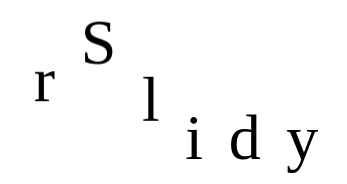
\includegraphics[width = .5\textwidth]{images/loading.png}	
	\caption[Loader]{
		Screenshot of the loading animations midway. On the left we see the inspirational pulz loader, while on the right we see the resulting rearrangement for \textit{rSlidy}.
		\imgcredit{Screenshot taken by the authors of this report.}
	}
	\label{fig:loading}
\end{figure}

% section initialization (end)

\section{Button Animation} % (fold)
\label{sec:button_animation}

Similar to an animated hamburger icon, which changes its shape on click, the buttons within the status bar of \textit{rSlidy} are animated now as well. Listing \ref{list:buttonflip} shows how the animated flip was created. These style changes and the button's text changed to an "X" lead to a simple and intuitive animation of a button which turns around to change its functionality. While the animation is done in CSS, the text change is done by the JavaScript setTimeout, to change the value halfway through the animation, when the text is not visible.
\begin{minipage}{\linewidth}
	\begin{lstlisting}[
	language=CSS,
	label=list:buttonflip,
	caption={[Flip Button Animation] Implementation of the animation of the buttons in the status bar
	}
	]
#button-overview, #button-toc, #button-menu{ 
	animation-duration: 0.3s; 
	animation-timing-function: ease-in-out;
	animation-fill-mode: forwards;
	animation-name: flip2Face;
}

#button-overview.clicked, #button-toc.clicked, #button-menu.clicked{
	animation-name: flip2Back; 
	transform: rotateY(180);
}
	\end{lstlisting}
\end{minipage}

\subsection{Same Element Animation Issue} % (fold)
\label{sub:same_element_animation_issue}

By having a direction and play animation property it seems that there is no need for two keyframe definitions, as in code snipplet \ref{list:buttonflip}. However getting it to work on same element is another issue. By researching forums, the main issue lies in the nature of CSS, overlaping properties from previous class, which seems to include counters. This becomes troublesome, when animation count is not infinite, like with button rotations example. While a simple transition would work if it was just a rotation, including a bit of scaling in the middle of the transformation to get a better effect, makes it impossible to solve with transitions. This issue became also a problem in section \ref{sec:slide_transitions}. The best pure CSS solution solution without adding additional HTML elements or doing JS animation was to actually write a reverse keframe copy and use that name in the needed class, which seems to reset the counter due animation initialization.

% subsection same_element_animation_issue (end)

% section button_animation (end)

\section{Hiding Elements} % (fold)
\label{sec:hiding_elements}

While hiding elements on hover elements by itself already raises the user experience, just by adding simple transition or animation CSS element we can direct the switch between states into a smooth way to enhance the user workflow. For better control we also used the Cubic Bezier function, with the values shown in figure \ref{fig:cubic-bezier}.

\begin{figure}[tp]
	\centering
	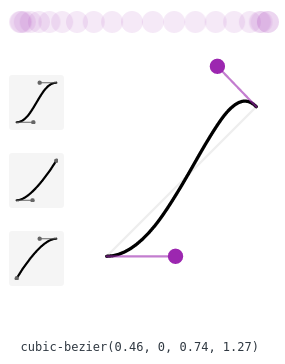
\includegraphics[width = .4\textwidth]{images/cubic-bezier.png}
	
	\caption[Cubic Bezier Function]{
		The values of the Cubic Bezier function used for smoother hiding of elements and its plot representation
		\imgcredit{Screenshot of the representation in Chrome Developer Tools taken by the authors of this report.}
	}
	\label{fig:cubic-bezier}
\end{figure}

% section hiding_elements (end)

\section{Preview Scrolling} % (fold)
\label{sec:preview_scrolling}

The Slides previous most of the time give you a nice preview of the slides. However depending on the amount of text or even the screen size due to using proportions for the thumbnails the preview may not be clear enough which slide it is due to the text overflow being hidden. Therefore we added a simple on hover animation of translating the thumbnail content by 20\% upwards. The only thing also to note was the choosing of the correct content to move. Namely moving the first child also moves the afixed click event, while further children had problems with z-indecies. Understanding the z-index property and the structure of your CSS code is the key for such situations. A great by-product of an on hover animation is that is a great indicator for the current mouse position, which the original \textit{rSlidy} on hover event only covered by slightly changing the color.

% section preview_scrolling (end)thumbnail
\newpage
\section{Slide Transitions} % (fold)
\label{sec:slide_transitions}

The last described animation was also the biggest contribution for a more dynamic presentetion flow. The goal was to include a simple way for the user to chose animated transitions between slides. To keep the previous version of immediate transitions also as an option of \textit{rSlidy}, we simply defined a body class \textit{animated}, on which all animated transition classes are referenced through.

First problem we faced was the original definition of \textit{hidden}, that uses display property set to none. This sets the the element not to be included in the render list of the browser, which however is required for animations to be applied. Since the display property is uncompatible with animation and the hiding of slides is the core of the application, we redefined the the \textit{hidden} for \textit{animated} bodies. The new definition uses visibility and sizes switched to hidden and 0 to achieve similar result as display set to none, while keeping it in the rendering list. Sadly this also means, that all animation keyframe definitions get a suffix for the reseting of this properties to keep the design intact. Since the suffix was needed, it made a much easier to read implementation by defining all slides as hidden and to get the end state of an animation as the afterstate, compared to to defining extra classes or making the code even complexer.

For a slide transition we defined the interchanging slides as \textit{previous} and \textit{active}. The former being the start of the animation, at the start time became marked as \textit{hidden}, while the latter is the only slide that at the same time became without the \textit{hidden} class. Since the \textit{previous} slide is one of many \textit{hidden} slides, the core function \textit{showSlide} had to be slightly modified in its loop over the slides to keep the index of \textit{previous} in memory. This was achieved with the classes \textit{animate}, \textit{animatedForward}, \textit{animatedBackwards}. The first class is the marker class, while the remaining ones define the direction of the transition of \textit{previous} and \textit{active} slides. Each is asserted by the increase or decrease of the slide index. In the definition we see, that with no change in index there should be no animation. This is needed, since the change in hash tag in the URL also triggers \textit{showSlide}. The cases when it is needed is in case of initial loading, refreshing and manual change of slide by address. However, each click to the next or previous slide also changes the hash tag. Since we do not want triggering the animation on initialization, refresh or update after next and previous was processed already, the absence of direction classes does not trigger transitions. Therefore all transition definitions become a combination transition name and direction classes, that use one of the defined keframes. The primary reason for direction classes was however creation of complex animation where the direction flow has to be followed to not confuse the observer. For example if slides go all to the right, if we step back we would like to see them move backwards or in other words to the left.


\begin{minipage}{\linewidth}
	\begin{lstlisting}[
	language=CSS,
	label=list:transitionMain,
	caption={[Transition Animation] Redefinition of hidden on all slides, an example of a keyframe with suffix due to the redefinition and general animation settings for animated transitions.
	}
	]
body.animated .slide{
	display: block;
	overflow: hidden;
	visibility: hidden;
	height: 0;
	width: 0;
	padding: 0;
}

@keyframes opacityOff{
0%	{opacity: 1; visibility: visible; height: auto; width: auto; padding: 2em;}
99%	{opacity: 0; visibility: visible; height: auto; width: auto; padding: 2em;}
100%{opacity: 0; visibility: hidden; height: 0; width: 0; padding: 0;}
}
@keyframes opacityOn{
0%	{opacity: 0; visibility: hidden; height: 0; width: 0; padding: 0;}
1%	{opacity: 0; visibility: visible; height: auto; width: auto; padding: 2em;}
100%{opacity: 1; visibility: visible; height: auto; width: auto; padding: 2em;}
}
@keyframes opacityOnList{
0%	{opacity: 0; visibility: hidden; height: 0;	width: 0;}
1%	{opacity: 0; visibility: visible; height: auto; width: auto;}
100%{opacity: 1; visibility: visible; height: auto; width: auto;}
}

/* General transition animation settings */
body.animated .slide,
body.animated .slide ul.incremental li:not(.invisible){
	animation-fill-mode: forwards;
	animation-duration: 1s;
	animation-timing-function: linear;
}
body.animated .slide ul.incremental li:not(.invisible){
	animation-fill-mode: backwards;
}
/* Without direction we skip the animation*/
body.animated :not(.animatedForward):not(.animatedBackwards).slide{
	animation-duration: 0s;
	/* for loader preloading it is set to the minimum JS 1ms delay*/
	animation-delay: 0.001s;
}
/* TIME DELAY FOR NEW SLIDE SHOULD BE SAME AS TRANSITION DURATION*/
body.animated :not(.hidden).slide{
	animation-delay: 1s;		
}

	\end{lstlisting}
\end{minipage}

Since the definition of classes was done rather long and complex, the result in the slide HTML file is, that the user has just ot append the transition class name either in the body class as a gloabal setup or in slide or list class for local setup. The prepared 
animated transition sum up to six: \textit{opacity, scale, sliding-left, sliding-right, sliding-left-right, sliding-right-left}. Their meaning should be clear from the words and for extra clarification see figure \ref{fig:transitions}. To make it more distincted for the user and easier to read the HTML slide file, the global and local seperation is done even in the class name, by apending \textit{-animation} to the name. For example the defualt global transition (when no transition name was referenced but \textit{animated} body was used) \textit{opacity}, becomes locally \textit{opacity-animation}.

\begin{minipage}{\linewidth}
	\begin{lstlisting}[
	language=CSS,
	label=list:transitionOpacity,
	caption={[Default Transition Animation] The default opacity transition is simple example of needed binding of HTML elements, transition names, directions and transition keyframes.
	}
	]
/************************************************/
/*			DEFAULT OPACITY transition			*/
/************************************************/
/* General animation settings for old slide */
body.animated .hidden.slide.animate,
/* Also sets the calls for default animation of opacity change */
body.animated.opacity .hidden.slide.animate,
body.animated .hidden.slide.animate.opacity-animation{
	animation-name: opacityOff; /* Default animation */
}

/* General animation settings for new slide */
body.animated :not(.hidden).slide,
/* Also sets the calls for default animation of opacity change */
body.animated.opacity :not(.hidden).slide,
body.animated :not(.hidden).slide.opacity-animation{
	animation-name: opacityOn; /* Default animation */
}

body.animated .slide ul.incremental li:not(.invisible),
body.animated.opacity .slide ul.incremental li:not(.invisible),
body.animated .slide.opacity-animation ul.incremental li:not(.invisible),
body.animated .slide ul.incremental.opacity-animation li:not(.invisible){
	animation-name: opacityOnList; /* Default animation */	
}
	\end{lstlisting}
\end{minipage}


\subsection{Solution Limitations} % (fold)
\label{sub:solution_limitations}

As noted in section \ref{sub:same_element_animation_issue}, one execution count animations have problems reversing the keframes for backwards direction. Additionally next to copying the code for the reverse keframe, one has to keep in mind that visibility property is a binary value and cannot be interpolated. An extra copy of keframes is also needed for the list animation, since lists use different padding than the slide keframe suffix. Another drawback in the actual execution of costum transitions is, that atmost 1 slide has sizes different than 0. This means we have to wait for the previous slide to become hidden before the active animation should start. This guideline secures, that the slide position will not jerk in the middle of transition due to the size changes of the other slide. There should be a possible solution, for exmaple with z-index and absolute postion redefiniton, however we ran out of time to test such ideas.

% subsection solution_limitations (end)

\begin{figure}[tp]
	\centering
	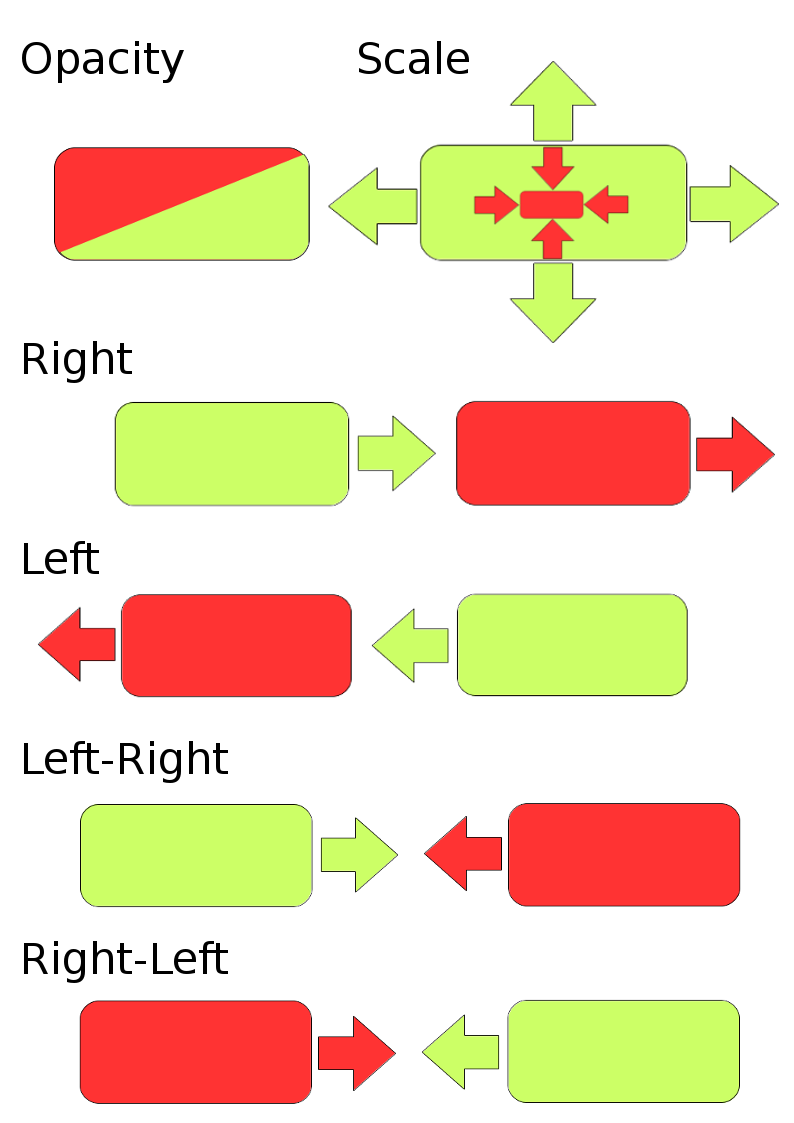
\includegraphics[width = .9\textwidth]{images/transitions.png}
	
	\caption[Slide Transition Diagram]{
		Diagram of \textit{rSlidy} included transitions and their flow. Red slides are the previous slides, while green are active slides. The position of active and previous slide is shown as relative position to the other.
		\imgcredit{Diagram is prepared by the authors of this report.}
	}
	\label{fig:transitions}
\end{figure}

% section slide_transitions (end)